\documentclass[12pt]{article}
\usepackage{amsmath, esint}
\usepackage{amsthm}
\usepackage{amsfonts}
\usepackage{amssymb}
\usepackage{enumerate}
\usepackage{tikz}
\usepackage[margin = .75in]{geometry}
\pagestyle{empty}

\newcommand{\Rr}{\mathbb{R}}
\newcommand{\ihat}{\hat{\textbf{i}}}
\newcommand{\jhat}{\hat{\textbf{j}}}
\newcommand{\flow}[1]{\par\noindent\textit{#1}\par\vspace{1mm}}
\newcommand{\drawgrid}{%
\begin{center}
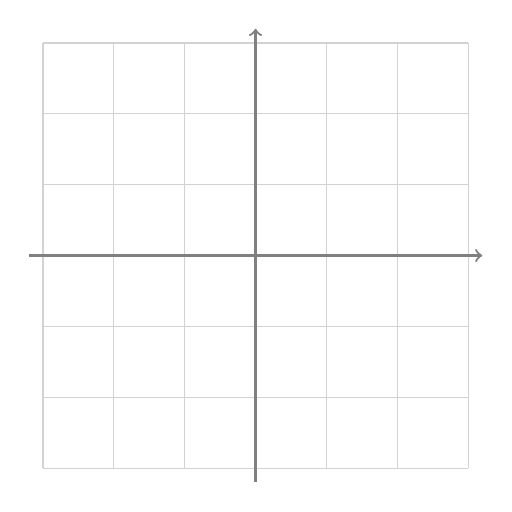
\begin{tikzpicture}[scale=0.9]
  \draw[step=1, gray!35, thin] (-3,-3) grid (3,3);
  \draw[gray, thick, ->] (-3.2,0) -- (3.2,0);
  \draw[gray, thick, ->] (0,-3.2) -- (0,3.2);
\end{tikzpicture}
\end{center}}

\begin{document}
\raggedright
\begin{center}
  {\large Worksheet. Vector Fields from Two Directions}\\
  \vspace{5mm}
\end{center}

\section*{Part A. What does an integral measure? (about 45 minutes)}

\flow{Every integral has a domain and an integrand. First see what integrating $1$ does.}

\begin{enumerate}
  \item Compute $\displaystyle\int_2^5 dx$. No integrand, just $dx$. What geometric feature of the interval $[2,5]$ does your answer measure?
  \item Now put a function inside, $\displaystyle\int_2^5 f(x)\,dx$ for a positive $f$. What does the integral measure now? In one sentence, what did inserting $f$ do to the meaning? Think of $f$ as a weight attached to each point of the interval.
  \item Let $D$ be the unit disk in the plane. Without computing anything, say what $\displaystyle\iint_D dA$ measures, and write down its value.
  \item Same disk, integrand inserted, $\displaystyle\iint_D f(x,y)\,dA$ with $f \geq 0$. What does this measure? Check your answer on the constant function $f = 3$. The disk has area $\pi$, so the integral should come out to a number you can defend with a picture of a very short cylinder.
  \item One more rung. $E$ is a solid region in space. What does $\displaystyle\iiint_E dV$ measure? And if $\rho(x,y,z)$ is the density of the material at each point, what does $\displaystyle\iiint_E \rho\,dV$ measure?
  \item Fill in the pattern. Integrating $1$ over a domain gives the \underline{\hspace{2cm}} of the domain. Integrating a function $f$ over the domain gives a \underline{\hspace{2cm}} total, where each piece of the domain counts with weight $f$. Notice the pattern held for one, two, and three dimensional domains.
  \item Here is the move the whole worksheet turns on. Let $C$ be a curved path in the plane, and write $ds$ for a tiny piece of its length. Following the pattern above, propose meanings for
  $$\int_C ds \qquad \text{and} \qquad \int_C f(x,y)\,ds.$$
  For the second one, two pictures are available. If $f$ is the linear density of a wire bent into the shape $C$, the integral is the wire's total \underline{\hspace{2cm}}. If instead $f(x,y)$ is the height of a fence built along $C$, the integral is the fence's \underline{\hspace{2cm}}.
\end{enumerate}

\section*{Part B. Fields of arrows (about 45 minutes)}

\flow{You already know a machine that eats a point and returns a vector.}

\begin{enumerate}\setcounter{enumi}{7}
  \item Let $f(x,y) = x^2 + y^2$, a bowl shaped terrain. Compute $\nabla f$ at the points $(1,0)$, $(0,1)$, $(-1,0)$, $(1,1)$, and $(2,0)$. On the grid below, draw each answer as an arrow based at its point.
  \drawgrid
  \item What you just drew is a \textbf{vector field}, a function $\vec F : \Rr^2 \to \Rr^2$ drawn by basing the arrow $\vec F(x,y)$ at the point $(x,y)$. In your own words, what does the gradient field of a terrain tell a hiker standing at each point?
  \item Now draw a field handed to you as a formula rather than born from a terrain. On the grid below, sketch $\vec F(x,y) = \langle -y,\, x \rangle$ at the eight points $(\pm 1, 0)$, $(0, \pm 1)$, $(\pm 1, \pm 1)$. Describe the overall motion in one word.
  \drawgrid
  \item On the same grid in a different mark, sketch $\vec G(x,y) = \langle x,\, y \rangle$ at the same eight points. How is $\vec G$ related to the arrows you drew in problem 8?
  \item Match each formula to its picture without plotting. Justify each match with one sentence.\\
  (i) $\langle 1, 0 \rangle$ \quad (ii) $\langle y, 0 \rangle$ \quad (iii) $\langle -x, -y \rangle$ \quad (iv) $\langle -y, x \rangle$\\
  (a) everything drains into the origin \quad (b) steady wind blowing east \quad (c) rotation about the origin \quad (d) eastward shear, faster the higher you stand, reversed below the axis
  \item Back to the bowl $f = x^2 + y^2$. Its level curves are circles centered at the origin. Add a few of them lightly to your grid from problem 8. What angle do the gradient arrows make with the level curves? Explain why it must be so. Walking along a level curve changes $f$ by nothing, and the gradient is the direction of fastest change.
  \item A field born as a gradient drags its terrain along behind it. Look at your two drawings, $\vec F = \langle -y, x\rangle$ and $\vec G = \langle x, y \rangle$. For each, could there be a terrain whose gradient it is? Do not decide yet. Write down one piece of evidence for or against each, and carry the question into Part D.
\end{enumerate}

\section*{Part C. Integrating along curves (about 45 minutes)}

\flow{Part A ended with integrals over curves. Part B handed us fields of arrows. Now put an arrow field under a curve integral.}

\begin{enumerate}\setcounter{enumi}{14}
  \item Warm up with the empty integrand. $C$ is the upper half of the unit circle. Write down $\displaystyle\int_C ds$ using a fact you have known since grade school. No parametrization allowed.
  \item A force $\vec F$ pushes an object along a straight displacement $\vec d$. From physics, the work done is $W = \vec F \cdot \vec d$. Why does only the component of $\vec F$ along $\vec d$ count? What is the work when $\vec F \perp \vec d$?
  \item Now the path curves and the force changes from point to point. Chop $C$ into tiny nearly straight steps $\Delta\vec r$. Write the work done over one step, then assemble the total as a limit of sums. You have just invented
  $$W = \int_C \vec F \cdot d\vec r.$$
  Nothing on the right is new. It is problem 7's curve integral with the integrand $\vec F \cdot \vec T$, the tangential component of the field.
  \item Compute by pure reasoning, no parametrizations. The field is $\vec F = \langle 0, -1 \rangle$, gravity pointing down with strength 1.\\
  (a) Work along the straight segment from $(0,0)$ to $(3,0)$.\\
  (b) Work along the straight segment from $(0,0)$ to $(0,-2)$.\\
  (c) Work along the straight segment from $(0,0)$ to $(3,-2)$. Explain the sign of each answer before you write it.
  \item The payoff of drawing. Take $\vec F = \langle -y, x \rangle$ and let $C$ be the unit circle traversed counterclockwise. At each point of $C$, compare the direction of $\vec F$ with the direction of travel, and compute $|\vec F|$ on the circle. Conclude that $\vec F \cdot d\vec r = ds$ along this path, and evaluate $\displaystyle\oint_C \vec F \cdot d\vec r$ with zero computation.
  \item Same circle, the radial field $\vec G = \langle x, y \rangle$. Evaluate $\displaystyle\oint_C \vec G \cdot d\vec r$ by pure geometry. One sentence.
  \item A general moral from the last two problems. The line integral of a field along a curve only sees the \underline{\hspace{2cm}} component of the field. A field everywhere perpendicular to your path does no \underline{\hspace{2cm}} on you.
\end{enumerate}

\section*{Part D. Conservative fields and the Fundamental Theorem (about 45 minutes)}

\flow{Part B left a question open. Which arrow fields are gradients of a terrain?}

\begin{enumerate}\setcounter{enumi}{21}
  \item A field $\vec F$ is \textbf{conservative} if $\vec F = \nabla f$ for some scalar function $f$, called a \textbf{potential} for $\vec F$. Find a potential for $\vec G = \langle x, y \rangle$ by inspection. Check it by taking the gradient.
  \item Level curves cannot cross. Suppose two different level curves of a function $f$ passed through the same point $P$. What two different values would $f(P)$ have to take? Conclude. At a point where $\nabla f = \vec 0$ level sets can pinch, think of the very bottom of the bowl, but away from such points crossing is forbidden.
  \item Now suppose, hoping for a contradiction, that $\vec F = \langle -y, x \rangle$ had a potential $f$. By problem 13, the level curves of $f$ would run perpendicular to the arrows of $\vec F$ at every point. On your drawing from problem 10, sketch curves that cross every arrow at a right angle. What family of curves do you get, and at which point do all of them insist on meeting? Explain why problem 23 finds this rude.
  \item The same catastrophe, seen dynamically. Walk once counterclockwise around the unit circle. By problem 19, at every single step $\vec F \cdot d\vec r = ds > 0$. If $\vec F$ were $\nabla f$, each step would raise the value of $f$. You return to your starting point having strictly climbed the entire way. Write the resulting inequality about $f$ at the starting point, and enjoy the contradiction. So $\langle -y, x \rangle$ is not conservative, now proved two ways.
  \item \textbf{Fundamental Theorem of Line Integrals.} If $f$ has continuous gradient on a region containing the curve $C$ from point $A$ to point $B$, then
  $$\int_C \nabla f \cdot d\vec r = f(B) - f(A).$$
  Set this next to the Fundamental Theorem of Calculus, $\int_a^b f'(x)\,dx = f(b) - f(a)$. Identify the role of each ingredient. What plays the part of $f'$, of $a$ and $b$, of the interval?
  \item Use the theorem. With $\vec G = \langle x, y \rangle$ and your potential from problem 22, compute the work done by $\vec G$ along any path from $(1,0)$ to $(0,3)$. Then take a wildly different path between the same two points and compute again. What just happened, and why does the word conservative fit?
  \item Closed loops. Use the theorem to show that a conservative field does zero work around any closed loop. Then reconcile with problem 19, where the loop integral of $\langle -y, x \rangle$ was $2\pi$. You now hold three proofs that the rotation field has no potential. Name all three in one line each, crossing contours, the ever climbing hike, the nonzero loop.
  \item Last look backward. In problem 6 you said integrating $1$ measures the domain and integrating a function gives a weighted total. State what the Fundamental Theorem of Line Integrals says the weighted total $\int_C \nabla f \cdot d\vec r$ collapses to, and marvel briefly that the entire path drops out, leaving only the two endpoints.
\end{enumerate}

\end{document}
